\section{Virtual reality and Digital games lab.}
\subsubsection{Presentation}

With various virtual, augmented and mixed reality appliances, this lab aims to backup INSPER's Computer Engineering classes. In addition to supply students and professors from the community.

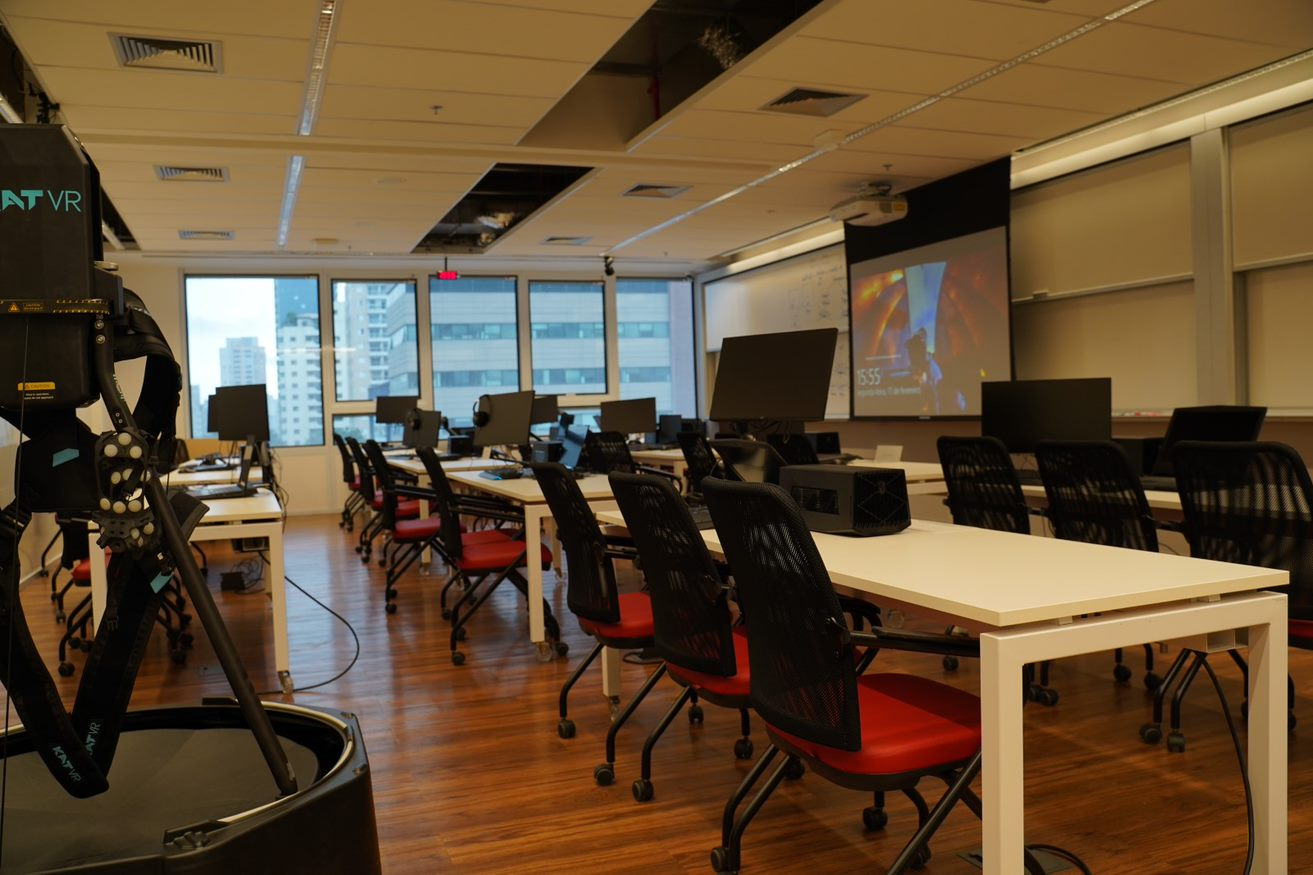
\includegraphics[width=\textwidth]{imgs/labrv.jpg}

The lab has max capacity of 36 students, in 12 workstations with 3 seats each. Every workstation has an 17R4 Alienware notebook, mechanical keyboard, high DPI mouse, Nvidia GeForce GTX1080 TI external graphics card, and a 24 inches full-HD Dell monitors.

Beyond the workstations the lab has several peripherals devices intended for digital games and extended reality development: 14 HTC Vive, 2 HTC Vive Pro, 1 Oculus Rift, 1 Hololens 1.0, 1 Magic Leap, 1 Vuzix Blade, 2 Google Daydream, 2 Touch Haptics, 3 Yoke Joysticks, 1 Force Feedback Driving Wheel, and many more.

In addition to the cited gadgets, the lab has multiple game consoles, 5 Xbox One, 1 Xbox One X, 1 Nintendo New3DS, 1 Nintendo Switch, 1 Google Pixel, 1 Samsung S9, 1 IPhone 12 Pro.

For video capture in 360 degrees, 180 degrees with or without stereoscopy, the lab has: 1 Rich Theta Camera, 1 LucidCam Camera, 1 WeeView Camera, and 1 Insta360 Pro.

Counts with structure for multimedia content production with: 1 Sony Alpha 7iii, 1 Green Chroma Key, Lighting Kit, Tripods, Microphones, 1 Huion Kamvas Digital Tablet, 1 Yamaha MG16XU Sound Mixer.

\newpage
\subsubsection{Objectives}

\begin{enumerate}
    \item Develop technical handling and use of motion capture devices, Head Mounted Displays and other Extended reality devices;
    \item Develop Virtual Reality and/or digital games applications;
    \item To use development platforms in creating new applications;
    \item Develop projects using programming languages (C\#, C++, Python, and others)
    \item Develop projects with graphical engines (Unity, Unreal, and others)
    \item Develop technical art skills comprehending 3D modeling, texturing, rigging and animation
\end{enumerate}
\newpage


\subsubsection{Security Policy}
\begin{enumerate}
    \item It is not allowed to eat food inside the lab;
    \item It is not allowed to drink beverages in open containers;
    \item Do not use the power outlets except for plugging lab equipment or personal notebook;
    \item In any doubt on equipment handling, ask for technical support;
    \item INSPER exempts it's responsibility over personal equipment connected to institution equipment.
    \item The lab's computers must be used only for application development and other disciplines related projects;
    \item All power outlets are 220V;
    \item {\color{red}IN EMERGENCIES CALL 9 FROM ANY EXTENSION LINE; In case of accident, look immediately the professor or technician, even in case of apparent no harm.}
\end{enumerate}

\subsubsection{Internal Procedures}
\begin{enumerate}
    \item It is not allowed to stay in the lab's dependencies without a technician or professor;
    \item It is not allowed the withdraw any equipment without previous authorisation by a technician or professor; 
    \item Do not install any software without team authorisation;
    \item Do not move any kept equipment without team authorisation;
\end{enumerate}

\newpage
\subsection{Disciplines}

\subsubsection{Digital Games - $7^{th}$ semester} 

Game typology; Digital games production process; Game Design; Level Design; Agile in digital games; Interaction Design for games; Game development technologies (GPU, graphical libraries, frameworks and engines); Game prototyping agile techniques; Assets production (Scenes, Models, Animations, Audio, Videos, Scripts); In game assets integration; Play-testing; Physical realism in games; Artificial Intelligence; Multiplayer games; Console Games; Publishing and marketing games; Business and entrepreneurship 
for games.

\subsubsection{Advanced Digital Games - Computer Engineering Elective}

Generic game engine structure; Game Engines Comparative Studies; Software Engineering for Games; Parallelism and Concurrency; Geometry Engines; Rendering Engines; Animation Engines; Audio Engines; Artificial Intelligence Engine; Network Engine; Game Engine Testing; Version management and code configuration of game engines;

\subsubsection{Virtual Reality - Computer Engineering Elective}

Virtual Reality; Sound and Graphical Components; Nature of interaction with the user in virtual ambience; Computer Graphics; Augmented Reality notions; Human-computer Interaction; Textures and Mapping; Geometric Transformations in two and three dimensions; Projective transformations; 3D Objects and Scenes definition; Animation and computer simulation; 3D Interaction; Lighting and shading models; Human Visual Perception; Stereoscopy; Interaction Devices; Real Time Interaction; Usability;

\subsubsection{Computational Vision - Computer Engineering Elective}

Basics of Computational vision, image processing and their Engineering applications; Main areas of computational vision and image processing; Image model (Source; Attributes; Models); Intensity transformation and special filtering; frequency domain filtering; Wavelets; Mathematical Morphology; characteristic detectors and descriptors; Similarity Estimation; Distances in the Feature Space; Camera model and geometric methods; Coordinate systems; Affine transformations; Projection matrix and perspective transformation; Pose estimation; Camera calibration; 3D Object Reconstruction; 

\newpage


\subsection{Our Team}
\setlength{\columnsep}{-10cm}
\begin{multicols}{2}
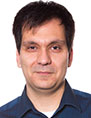
\includegraphics[width=3cm]{imgs/luciano-soares.jpg}
\columnbreak
\subsubsection{Luciano Pereira Soares - Lab. Coordinator}

Luciano Soares is an associate professor at Insper, having participated in the creation and implementation of the school's engineering programs. He is currently responsible for partnerships with companies in engineering programs, in the coordination of the Final Engineering Project, in the academic research fronts in engineering and in the coordination of the Virtual Reality and Digital Games laboratory.

Luciano Soares holds a degree in Computer Engineering from UFSCar, a PhD in Electrical Engineering from Escola Politécnica da USP and a post-doctorate from Instituto Superior Técnico (INESC/IST), Instituto Superior de Ciências do Trabalho e da Empresa (ADETTI/ISCTE) and Instituto Superior de Ciências do Trabalho e da Empresa (ADETTI/ISCTE) and Instituto Superior de Ciências do Trabalho e da Empresa (ADETTI/ISCTE). National de Recherche en Informatique et Automatique (INRIA), and holds an MBA in Project Management from FGV. He was a professor at the Department of Informatics at PUC-Rio, where he developed several research projects with Petrobras.

He develops research in the area of ​​Virtual Reality, where he was in charge of the design and construction of the Digital Cave, the first cubic multi-projection system (CAVE) in Brazil, and collaborated with the creation of the virtual reality centers of Lousal, Leme, NRCP/PUC- Rio and NVC/CENPES. He was also a systems engineer at Silicon Graphics Inc. and at Alias|wavefront and project manager at LSI-TEC and Tecgraf. Luciano Soares is the current president of the Special Committee on Virtual Reality of the Brazilian Computer Society.

\end{multicols}

\begin{multicols}{2}
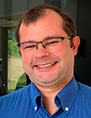
\includegraphics[width=3cm]{imgs/fabio-miranda.jpg}
\columnbreak
\subsubsection{Fabio Roberto de Miranda - Lab. Coordinator}

Coordinator of the Computer Engineering Course, Fabio de Miranda is an electrical engineer with an emphasis on Computing and a Master's degree in Electronic Systems from the Polytechnic School of USP. He is currently collaborating with the design of new engineering courses at Insper.
He develops applied research and produced system prototypes in the areas of Augmented Reality, Computer Graphics and Computer Vision. He provides consultancy on specification and development of graphic systems or systems with non-trivial requirements for institutions and companies in the market, including Embraer, CTI and Cenpes-Petrobras.

He has been teaching undergraduate and graduate courses in the area of information technology since 2001. He has supervised scientific initiation and course completion works and developed and coordinated a Computer Engineering course. He has experience in project-oriented disciplines that use resources such as simulators, mobile devices, physical computing, and educational robotics.

\end{multicols}

\begin{multicols}{2}
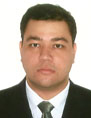
\includegraphics[width=3cm]{imgs/Raul-Ikeda.jpg}
\columnbreak
\subsubsection{Raul Ikeda Gomes da Silva - Lab. Coordinator}

Associate professor at Insper and manager of the Networks and Supercomputing Laboratory, Raul Ikeda Gomes da Silva holds a degree in Computer Science from the Universidade Estadual Paulista Júlio de Mesquita Filho (2001) and a master's degree in Electronic and Computer Engineering from the Technological Institute of Aeronautics (2003) .

He has professional experience in the financial market in Quantitative / High Frequency Trading, working on projects within fintechs and banks, specifically with modeling and process automation in real time. In recent years he has been working on research in the area of Computer Vision and Sensor Fusion to perform navigation of autonomous systems.

Research Area: Sensor Fusion, Quantitative Trading, Computer Vision.

\end{multicols}
\newpage
\begin{multicols}{2}
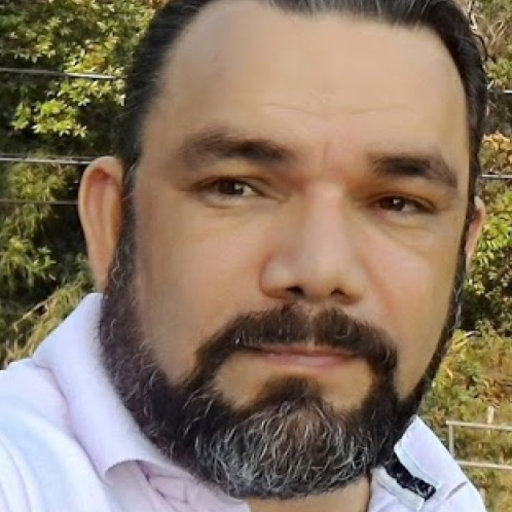
\includegraphics[width=3cm]{imgs/Luciano-Silva-17.jpg}
\columnbreak
\subsubsection{Luciano Silva - Professor}

Bachelor in Computer Science from the University of São Paulo (1996), Master in Applied Mathematics from the University of São Paulo (1998) and Doctor in Computer Science from the University of São Paulo (2004). His current research areas focus on Astroinformatics, High Performance Computing, Digital Game Design and Development, Virtual and Augmented Reality.

\end{multicols}

\begin{multicols}{2}
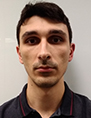
\includegraphics[width=3cm]{imgs/Igor-dos-Santos-Montagner.jpg}
\columnbreak
\subsubsection{Igor Montagner - Professor}

He holds a degree and a doctorate in Computer Science from the University of São Paulo, having completed a doctoral internship in France (INSA-Rouen). His thesis combined elements of Image Processing, Machine Learning and Linear Optimization aiming at the automatic creation of image segmentations.

He is currently a professor in the Computer Engineering course, working in disciplines in the Systems core. His recent research interests include the application of the data analysis methods studied in his PhD in the areas of accessibility and teaching in computing.

\end{multicols}

\begin{multicols}{2}
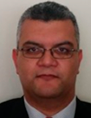
\includegraphics[width=3cm]{imgs/fabio-ayres.png}
\columnbreak
\subsubsection{Fábio Ayres - Professor}

Fábio Ayres is an associate professor at Insper, involved in the development of engineering courses. He holds a bachelor's and master's degree in Electrical Engineering from Escola Politécnica da USP and a PhD in Electrical Engineering from the University of Calgary, Canada. He was a postdoctoral fellow in Biomedical Engineering from the University of Calgary, Research Associate at the National Research Council of Canada, Software Engineer at Opal-RT Technologies, Canada, and Google. Interested in computer vision, machine learning, image processing, information retrieval, high-performance computing.

\end{multicols}

\begin{multicols}{2}

\includegraphics[width=3cm]{imgs/emil-freme.png}
\columnbreak
\subsubsection{Emil Freme - Lab. Technician}
Emil Freme is an assistant at the Virtual Reality and Digital Games Laboratory at Insper, a Digital Games student at Fatec São Caetano do Sul and iOS specialist at the Bepid Instituto Eldorado campus, also a Technical Artist at SAGA.

He has worked as a developer in several areas such as front-end, back-end, iOS, QA and Game Dev.


\end{multicols}

\newpage
\section{Equipment}
\setlength{\columnsep}{0.5cm}
\newcolumntype{Y}{>{\centering\arraybackslash}X}
%%%%%%%%%%%%%%%%%%%%%%%%%%%%%%%%%%%%%%%%%%%%%%%%%%%%%%%%%%%%%%%%%%%%%%%%%%%%%%%%%%%%%%%%%%
%%%%%%%%%%%%%%%%%%%%%%%%%%%%%%%%%%%%%%%%%%%%%%%%%%%%%%%%%%%%%%%%%%%%%%%%%%%%%%%%%%%%%%%%%%
%%%%%%%%%%%%%%%%%%%%%%%%%%%%%%%%%%%%%%%%%%%%%%%%%%%%%%%%%%%%%%%%%%%%%%%%%%%%%%%%%%%%%%%%%%
\subsection{Workstation}
\begin{tabularx}{\textwidth}{ Y  Y  Y  Y }
    \textbf{Description} &  \textbf{Local} &  \textbf{Quantity} & \textbf{Patrimony}\\
    \hline \\
     Demo station & Cart & 1 & Activated
\end{tabularx}
\vspace{1cm}

\begin{multicols}{2}

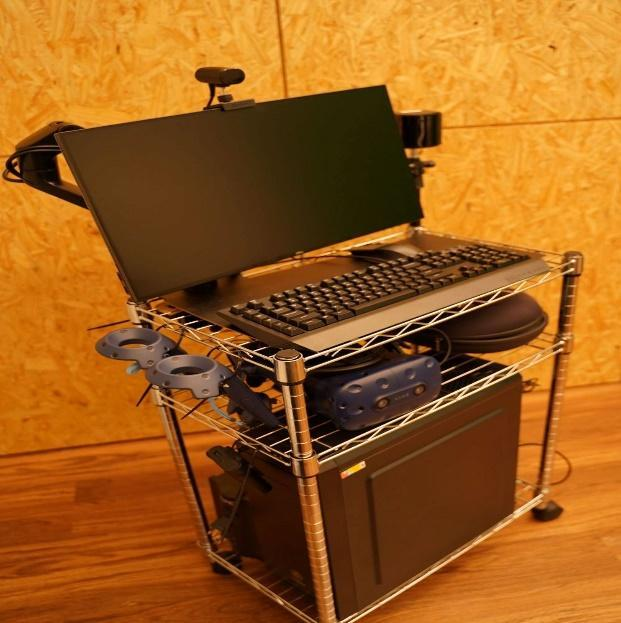
\includegraphics[width=80mm, keepaspectratio]{imgs/image3.jpg}

\columnbreak

\begin{mdframed}[roundcorner=10pt, linecolor=red, linewidth=2pt]
\vspace{1em}
{\Large {\color{red}RISKS}}
\vspace{1em}

\begin{itemize}
    \item Electric Chock;
    \item Equipment Damage;
    \item Physical Damage;
    \item Visual Fatigue; 
\end{itemize}

\vspace{1em}
\end{mdframed}

\vspace{2em}

{\Large Use}
\vspace{1em}

Allowed only with a technician or professor guidance.
\end{multicols}

{\Large Specs}
\vspace{1em}

\textbf{Processor:} Intel i9-9900k 3.6GHz; \textbf{RAM:} 36GB; \textbf{Graphics Card:} NVidia GeForce RTX 2080 TI 11GB VRAM; \textbf{Storage:} 250GB SSD + 2TB HDD;
\newpage
%%%%%%%%%%%%%%%%%%%%%%%%%%%%%%%%%%%%%%%%%%%%%%%%%%%%%%%%%%%%%%%%%%%%%%%%%%%%%%%%%%%%%%%%%%
%%%%%%%%%%%%%%%%%%%%%%%%%%%%%%%%%%%%%%%%%%%%%%%%%%%%%%%%%%%%%%%%%%%%%%%%%%%%%%%%%%%%%%%%%%
%%%%%%%%%%%%%%%%%%%%%%%%%%%%%%%%%%%%%%%%%%%%%%%%%%%%%%%%%%%%%%%%%%%%%%%%%%%%%%%%%%%%%%%%%%
\subsection{Alienware notebooks}
\begin{tabularx}{\textwidth}{ Y  Y  Y  Y }
    \textbf{Description} &  \textbf{Local} &  \textbf{Quantity} & \textbf{Patrimony}\\
    \hline \\
     Alienware 17R4 & Workstations & 12 & Activated \\
     Alienware 17R4 & Cabinet & 2 & Activated \\
     Alienware 17R5 & Cabinet & 2 & Activated \\
     Alienware Area51 & Cabinet & 7 & Activated
\end{tabularx}
\vspace{1cm}

\begin{multicols}{2}

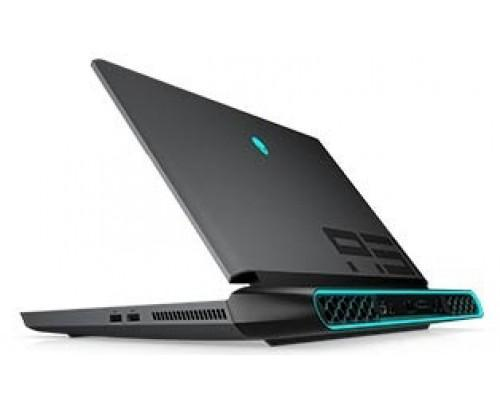
\includegraphics[width=60mm, keepaspectratio]{imgs/image4.jpg}

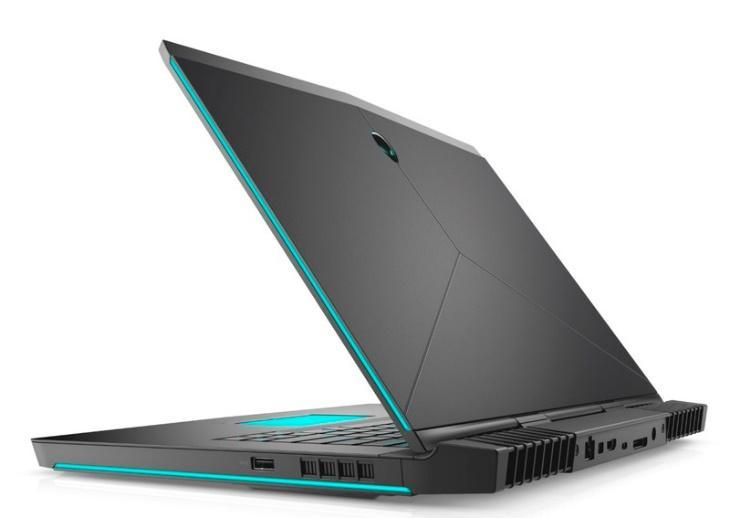
\includegraphics[width=60mm, keepaspectratio]{imgs/image5.jpg}

\columnbreak

\begin{mdframed}[roundcorner=10pt, linecolor=red, linewidth=2pt]
\vspace{1em}
{\Large {\color{red}RISKS}}
\vspace{1em}

\begin{itemize}
    \item Electric Chock;
    \item Equipment Damage;
    \item Physical Damage;
    \item Visual Fatigue; 
\end{itemize}

\vspace{1em}
\end{mdframed}

\vspace{2em}

{\Large Use}
\vspace{1em}

Allowed only with a technician or professor guidance;

Borrowing with previous authorisation; 

\end{multicols}

{\Large Specs}
\vspace{1em}

Alienware 17R4: \textbf{Processor:} Intel i7-7820k 2.90GHz; \textbf{RAM:} 36GB; \textbf{Graphics Card:} NVidia GeForce GTX 1080 8GB VRAM; \textbf{Storage:} 250GB SSD + 1TB HDD;

Alienware 17R5: \textbf{Processor:} Intel i9-8950k 2.90GHz; \textbf{RAM:} 36GB; \textbf{Graphics Card:} NVidia GeForce GTX 1080 8GB VRAM; \textbf{Storage:} 250GB SSD + 1TB HDD;

Alienware Area51: \textbf{Processor:} Intel i9-9900k 3.6GHz; \textbf{RAM:} 36GB; \textbf{Graphics Card:} NVidia GeForce RTX 2080 TI 11GB VRAM; \textbf{Storage:} 250GB SSD + 1TB HDD;
\newpage

%%%%%%%%%%%%%%%%%%%%%%%%%%%%%%%%%%%%%%%%%%%%%%%%%%%%%%%%%%%%%%%%%%%%%%%%%%%%%%%%%%%%%%%%%%
%%%%%%%%%%%%%%%%%%%%%%%%%%%%%%%%%%%%%%%%%%%%%%%%%%%%%%%%%%%%%%%%%%%%%%%%%%%%%%%%%%%%%%%%%%
%%%%%%%%%%%%%%%%%%%%%%%%%%%%%%%%%%%%%%%%%%%%%%%%%%%%%%%%%%%%%%%%%%%%%%%%%%%%%%%%%%%%%%%%%%
\subsection{Graphics Amplifier}
\begin{tabularx}{\textwidth}{ Y  Y  Y  Y }
    \textbf{Description} &  \textbf{Local} &  \textbf{Quantity} & \textbf{Patrimony}\\
    \hline \\
     Graphics Amplifier with NVidia 1080 Ti & Workstation & 14 & Activated
\end{tabularx}
\vspace{1cm}

\begin{multicols}{2}

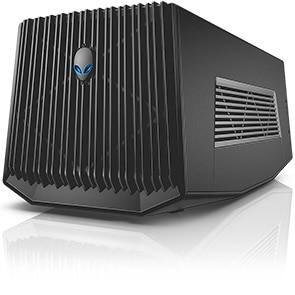
\includegraphics[width=80mm, keepaspectratio]{imgs/aga.jpg}

\columnbreak

\begin{mdframed}[roundcorner=10pt, linecolor=red, linewidth=2pt]
\vspace{1em}
{\Large {\color{red}RISKS}}
\vspace{1em}

\begin{itemize}
    \item Electric Chock;
    \item Equipment Damage;
\end{itemize}

\vspace{1em}
\end{mdframed}

\vspace{2em}

{\Large Use}
\vspace{1em}

Free to use in the workstations
\end{multicols}

{\Large Other Details}
\vspace{1em}

Driver: \url{https://www.dell.com/support/home/br/pt/brdhs1/drivers/driversdetails?driverid=wvjy2}

\newpage

%%%%%%%%%%%%%%%%%%%%%%%%%%%%%%%%%%%%%%%%%%%%%%%%%%%%%%%%%%%%%%%%%%%%%%%%%%%%%%%%%%%%%%%%%%
%%%%%%%%%%%%%%%%%%%%%%%%%%%%%%%%%%%%%%%%%%%%%%%%%%%%%%%%%%%%%%%%%%%%%%%%%%%%%%%%%%%%%%%%%%
%%%%%%%%%%%%%%%%%%%%%%%%%%%%%%%%%%%%%%%%%%%%%%%%%%%%%%%%%%%%%%%%%%%%%%%%%%%%%%%%%%%%%%%%%%
\subsection{HTC Vive / Pro}
\begin{tabularx}{\textwidth}{ Y  Y  Y  Y }
    \textbf{Description} &  \textbf{Local} &  \textbf{Quantity} & \textbf{Patrimony}\\
    \hline \\
     HTC Vive & Cabinet & 14 & Activated\\
     HTC Vive Pro & Cabinet & 2 & Activated
\end{tabularx}
\vspace{1cm}

\begin{multicols}{2}

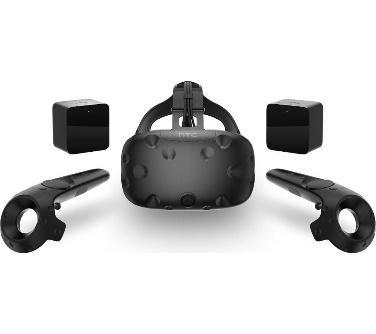
\includegraphics[width=60mm, keepaspectratio]{imgs/vive.jpg}

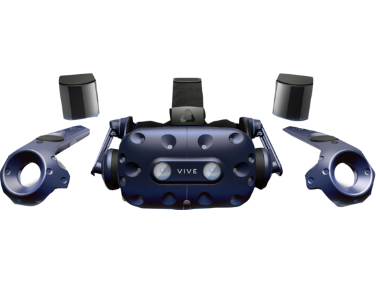
\includegraphics[width=60mm, keepaspectratio]{imgs/vivepro.png}

\columnbreak

\begin{mdframed}[roundcorner=10pt, linecolor=red, linewidth=2pt]
\vspace{1em}
{\Large {\color{red}RISKS}}
\vspace{1em}

\begin{itemize}
    \item Electric Chock;
    \item Equipment Damage;
    \item Physical Damage;
    \item Visual Fatigue; 
\end{itemize}

\vspace{1em}
\end{mdframed}

\vspace{2em}

{\Large Use}
\vspace{1em}

Can be borrowed with a technician or professor authorization.
\end{multicols}

{\Large Details}
\vspace{1em}

Every kit has: 
\begin{itemize}
    \item 1 Headset;
    \item 2 Joysticks
    \item 2 Base Stations (In the lab they are fixed in the ceiling)
    \item 1 Linkbox
\end{itemize}

\vspace{1em}
{\Large Other Details}
\vspace{1em}

Official Page: \url{https://www.vive.com/eu/}

Setup: \url{https://www.vive.com/eu/setup/}

Developer Portal: \url{https://developer.vive.com/eu/}
\newpage

%%%%%%%%%%%%%%%%%%%%%%%%%%%%%%%%%%%%%%%%%%%%%%%%%%%%%%%%%%%%%%%%%%%%%%%%%%%%%%%%%%%%%%%%%%
%%%%%%%%%%%%%%%%%%%%%%%%%%%%%%%%%%%%%%%%%%%%%%%%%%%%%%%%%%%%%%%%%%%%%%%%%%%%%%%%%%%%%%%%%%
%%%%%%%%%%%%%%%%%%%%%%%%%%%%%%%%%%%%%%%%%%%%%%%%%%%%%%%%%%%%%%%%%%%%%%%%%%%%%%%%%%%%%%%%%%
\subsection{Oculus Rift}
\begin{tabularx}{\textwidth}{ Y  Y  Y  Y }
    \textbf{Description} &  \textbf{Local} &  \textbf{Quantity} & \textbf{Patrimony}\\
    \hline \\
    Oculus Rift & Cabinet & 1 & Activated
\end{tabularx}
\vspace{1cm}

\begin{multicols}{2}

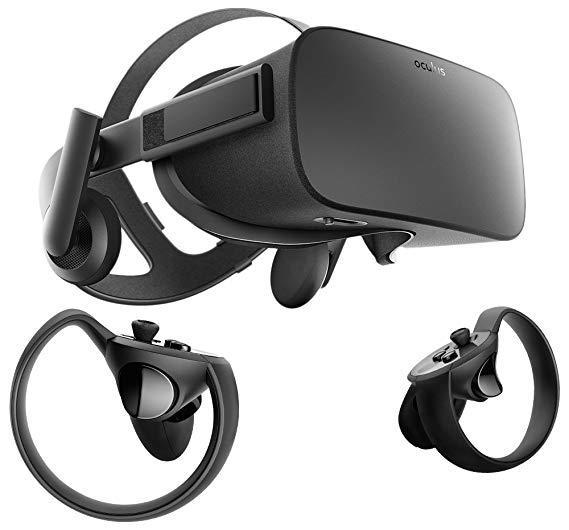
\includegraphics[width=80mm, keepaspectratio]{imgs/oculus.jpg}

\columnbreak

\begin{mdframed}[roundcorner=10pt, linecolor=red, linewidth=2pt]
\vspace{1em}
{\Large {\color{red}RISKS}}
\vspace{1em}

\begin{itemize}
    \item Electric Chock;
    \item Equipment Damage;
    \item Physical Damage;
    \item Visual Fatigue; 
\end{itemize}

\vspace{1em}
\end{mdframed}

\vspace{2em}

{\Large Use}
\vspace{1em}

Can be borrowed with a technician or professor authorization.
\end{multicols}

{\Large Other Details}
\vspace{1em}

Setup: \url{ https://support.oculus.com/857827607684748/}

Downloads: \url{https://developer.oculus.com/downloads/}

Docs: \url{ https://developer.oculus.com/documentation/}
\newpage


%%%%%%%%%%%%%%%%%%%%%%%%%%%%%%%%%%%%%%%%%%%%%%%%%%%%%%%%%%%%%%%%%%%%%%%%%%%%%%%%%%%%%%%%%%
%%%%%%%%%%%%%%%%%%%%%%%%%%%%%%%%%%%%%%%%%%%%%%%%%%%%%%%%%%%%%%%%%%%%%%%%%%%%%%%%%%%%%%%%%%
%%%%%%%%%%%%%%%%%%%%%%%%%%%%%%%%%%%%%%%%%%%%%%%%%%%%%%%%%%%%%%%%%%%%%%%%%%%%%%%%%%%%%%%%%%
\subsection{Augmented and Mixed Reality Glasses}
\begin{tabularx}{\textwidth}{ Y  Y  Y  Y }
    \textbf{Description} &  \textbf{Local} &  \textbf{Quantity} & \textbf{Patrimony}\\
    \hline \\
     Magic Leap & Cabinet & 1 & Activated \\
     Hololens & Cabinet & 1 & Activated \\
     Vuzix Blade & Cabinet & 1 & Activated
\end{tabularx}
\vspace{1cm}

\begin{multicols}{2}

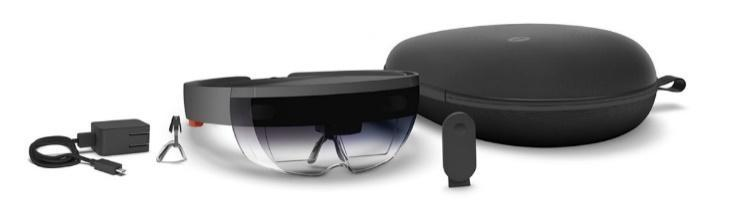
\includegraphics[width=60mm, keepaspectratio]{imgs/hololens.jpg}

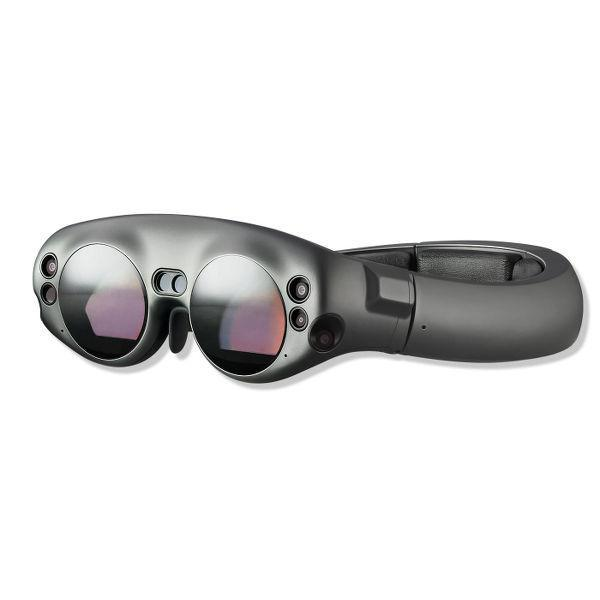
\includegraphics[width=60mm, keepaspectratio]{imgs/magicleap.jpg}

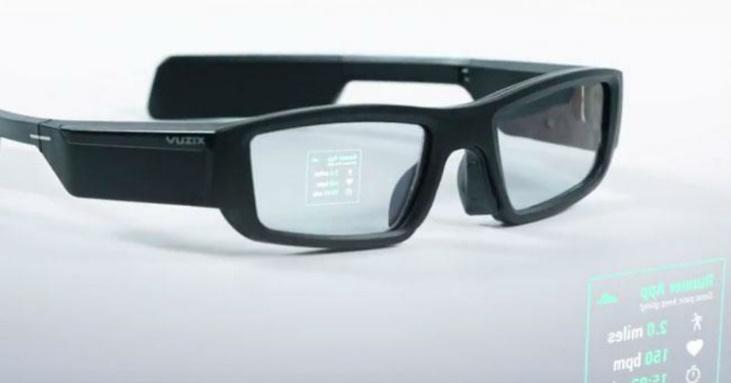
\includegraphics[width=60mm, keepaspectratio]{imgs/vuzix.jpg}

\columnbreak

\begin{mdframed}[roundcorner=10pt, linecolor=red, linewidth=2pt]
\vspace{1em}
{\Large {\color{red}RISKS}}
\vspace{1em}

\begin{itemize}
    \item Electric Chock;
    \item Equipment Damage;
    \item Physical Damage;
    \item Visual Fatigue;
    \item Burns
\end{itemize}

\vspace{1em}
\end{mdframed}

\vspace{2em}

{\Large Use}
\vspace{1em}

Allowed only with a technician or professor guidance.
\end{multicols}

{\Large Other Details}
\vspace{1em}

Hololens Hardware Details: \url{https://docs.microsoft.com/en-us/windows/mixed-reality/hololens-hardware-details}

Your First Hololens Mixed Reality Project: \url{https://docs.microsoft.com/en-us/windows/mixed-reality/holograms-100}

\vspace{1em}

Magic Leap Setup: \url{https://www.magicleap.care/hc/en-us/articles/360015853151-Getting-Started-with-Magic-Leap-One}

Magic Leap Dev. Portal: \url{https://creator.magicleap.com/learn/guides/creator-portal}

\vspace{1em}

Vuzix Setup: \url{https://bit.ly/3CCGtzL}

Vuzix Dev. Portal: \url{https://www.vuzix.com/Developers}

\newpage

%%%%%%%%%%%%%%%%%%%%%%%%%%%%%%%%%%%%%%%%%%%%%%%%%%%%%%%%%%%%%%%%%%%%%%%%%%%%%%%%%%%%%%%%%%
%%%%%%%%%%%%%%%%%%%%%%%%%%%%%%%%%%%%%%%%%%%%%%%%%%%%%%%%%%%%%%%%%%%%%%%%%%%%%%%%%%%%%%%%%%
%%%%%%%%%%%%%%%%%%%%%%%%%%%%%%%%%%%%%%%%%%%%%%%%%%%%%%%%%%%%%%%%%%%%%%%%%%%%%%%%%%%%%%%%%%
\subsection{Leap Motion}
\begin{tabularx}{\textwidth}{ Y  Y  Y  Y }
    \textbf{Description} &  \textbf{Local} &  \textbf{Quantity} & \textbf{Patrimony}\\
    \hline \\
     Demo station & Cart & 1 & Activated
\end{tabularx}
\vspace{1cm}

\begin{multicols}{2}

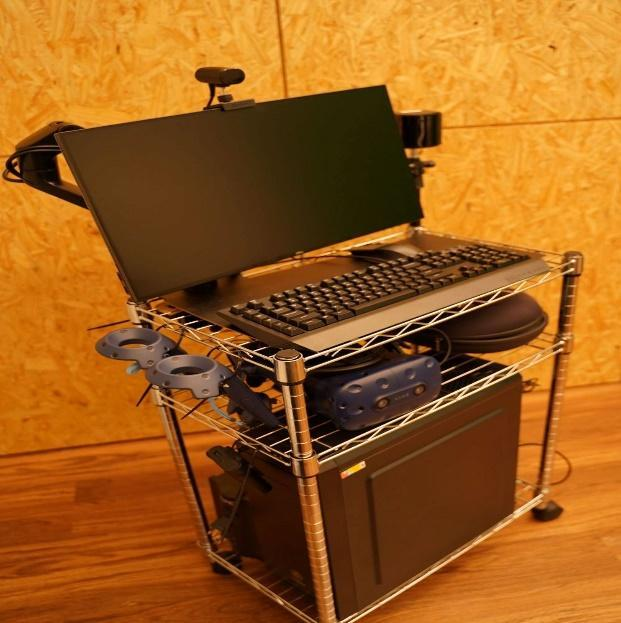
\includegraphics[width=80mm, keepaspectratio]{imgs/image3.jpg}

\columnbreak

\begin{mdframed}[roundcorner=10pt, linecolor=red, linewidth=2pt]
\vspace{1em}
{\Large {\color{red}RISKS}}
\vspace{1em}

\begin{itemize}
    \item Electric Chock;
    \item Equipment Damage;
    \item Physical Damage;
    \item Visual Fatigue; 
\end{itemize}

\vspace{1em}
\end{mdframed}

\vspace{2em}

{\Large Use}
\vspace{1em}

Allowed only with a technician or professor guidance.
\end{multicols}

{\Large Specs}
\vspace{1em}

\textbf{Processor:} Intel i9-9900k 3.6GHz; \textbf{RAM:} 36GB; \textbf{Graphics Card:} NVidia GeForce RTX 2080 TI 11GB VRAM; \textbf{Storage:} 250GB SSD + 2TB HDD;
\newpage

%%%%%%%%%%%%%%%%%%%%%%%%%%%%%%%%%%%%%%%%%%%%%%%%%%%%%%%%%%%%%%%%%%%%%%%%%%%%%%%%%%%%%%%%%%
%%%%%%%%%%%%%%%%%%%%%%%%%%%%%%%%%%%%%%%%%%%%%%%%%%%%%%%%%%%%%%%%%%%%%%%%%%%%%%%%%%%%%%%%%%
%%%%%%%%%%%%%%%%%%%%%%%%%%%%%%%%%%%%%%%%%%%%%%%%%%%%%%%%%%%%%%%%%%%%%%%%%%%%%%%%%%%%%%%%%%
\subsection{Video Game Consoles}
\begin{tabularx}{\textwidth}{ Y  Y  Y  Y }
    \textbf{Description} &  \textbf{Local} &  \textbf{Quantity} & \textbf{Patrimony}\\
    \hline \\
     Demo station & Cart & 1 & Activated
\end{tabularx}
\vspace{1cm}

\begin{multicols}{2}

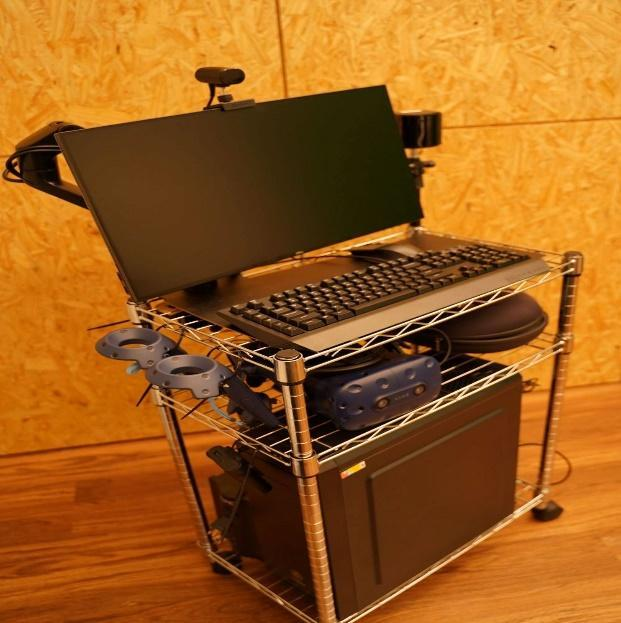
\includegraphics[width=80mm, keepaspectratio]{imgs/image3.jpg}

\columnbreak

\begin{mdframed}[roundcorner=10pt, linecolor=red, linewidth=2pt]
\vspace{1em}
{\Large {\color{red}RISKS}}
\vspace{1em}

\begin{itemize}
    \item Electric Chock;
    \item Equipment Damage;
    \item Physical Damage;
    \item Visual Fatigue; 
\end{itemize}

\vspace{1em}
\end{mdframed}

\vspace{2em}

{\Large Use}
\vspace{1em}

Allowed only with a technician or professor guidance.
\end{multicols}

{\Large Specs}
\vspace{1em}

\textbf{Processor:} Intel i9-9900k 3.6GHz; \textbf{RAM:} 36GB; \textbf{Graphics Card:} NVidia GeForce RTX 2080 TI 11GB VRAM; \textbf{Storage:} 250GB SSD + 2TB HDD;
\newpage

%%%%%%%%%%%%%%%%%%%%%%%%%%%%%%%%%%%%%%%%%%%%%%%%%%%%%%%%%%%%%%%%%%%%%%%%%%%%%%%%%%%%%%%%%%
%%%%%%%%%%%%%%%%%%%%%%%%%%%%%%%%%%%%%%%%%%%%%%%%%%%%%%%%%%%%%%%%%%%%%%%%%%%%%%%%%%%%%%%%%%
%%%%%%%%%%%%%%%%%%%%%%%%%%%%%%%%%%%%%%%%%%%%%%%%%%%%%%%%%%%%%%%%%%%%%%%%%%%%%%%%%%%%%%%%%%
\subsection{Kinect}
\begin{tabularx}{\textwidth}{ Y  Y  Y  Y }
    \textbf{Description} &  \textbf{Local} &  \textbf{Quantity} & \textbf{Patrimony}\\
    \hline \\
     Demo station & Cart & 1 & Activated
\end{tabularx}
\vspace{1cm}

\begin{multicols}{2}

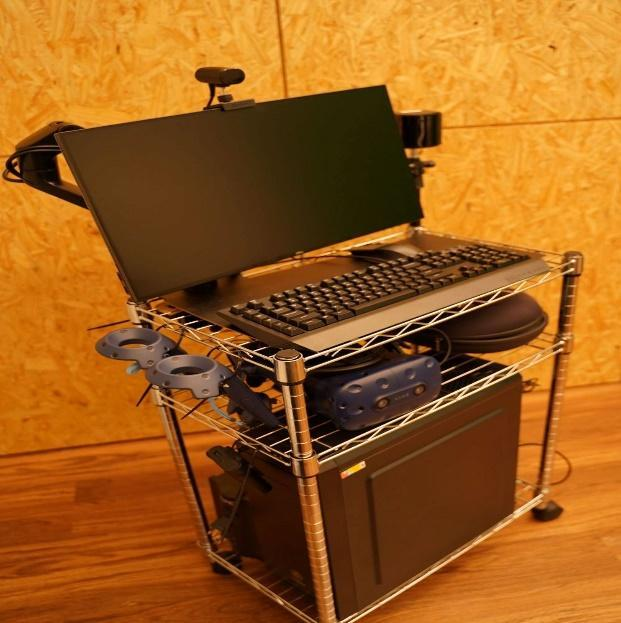
\includegraphics[width=80mm, keepaspectratio]{imgs/image3.jpg}

\columnbreak

\begin{mdframed}[roundcorner=10pt, linecolor=red, linewidth=2pt]
\vspace{1em}
{\Large {\color{red}RISKS}}
\vspace{1em}

\begin{itemize}
    \item Electric Chock;
    \item Equipment Damage;
    \item Physical Damage;
    \item Visual Fatigue; 
\end{itemize}

\vspace{1em}
\end{mdframed}

\vspace{2em}

{\Large Use}
\vspace{1em}

Allowed only with a technician or professor guidance.
\end{multicols}

{\Large Specs}
\vspace{1em}

\textbf{Processor:} Intel i9-9900k 3.6GHz; \textbf{RAM:} 36GB; \textbf{Graphics Card:} NVidia GeForce RTX 2080 TI 11GB VRAM; \textbf{Storage:} 250GB SSD + 2TB HDD;
\newpage

%%%%%%%%%%%%%%%%%%%%%%%%%%%%%%%%%%%%%%%%%%%%%%%%%%%%%%%%%%%%%%%%%%%%%%%%%%%%%%%%%%%%%%%%%%
%%%%%%%%%%%%%%%%%%%%%%%%%%%%%%%%%%%%%%%%%%%%%%%%%%%%%%%%%%%%%%%%%%%%%%%%%%%%%%%%%%%%%%%%%%
%%%%%%%%%%%%%%%%%%%%%%%%%%%%%%%%%%%%%%%%%%%%%%%%%%%%%%%%%%%%%%%%%%%%%%%%%%%%%%%%%%%%%%%%%%
\subsection{Wheel Joystick with force feedback}
\begin{tabularx}{\textwidth}{ Y  Y  Y  Y }
    \textbf{Description} &  \textbf{Local} &  \textbf{Quantity} & \textbf{Patrimony}\\
    \hline \\
     Demo station & Cart & 1 & Activated
\end{tabularx}
\vspace{1cm}

\begin{multicols}{2}

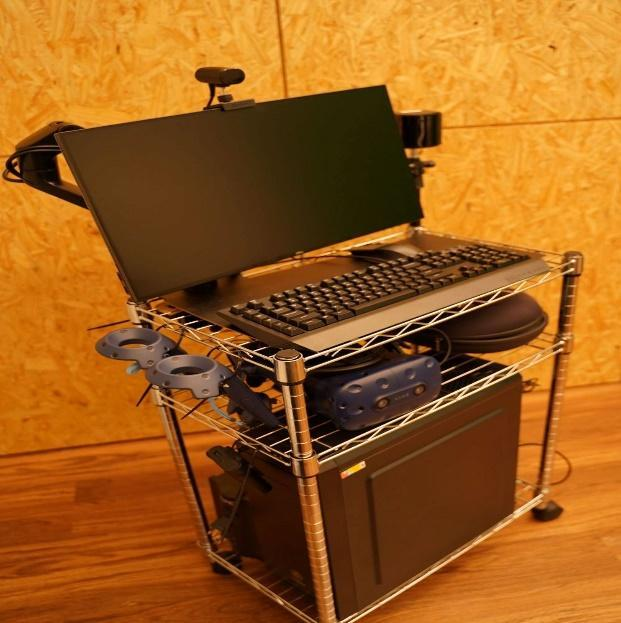
\includegraphics[width=80mm, keepaspectratio]{imgs/image3.jpg}

\columnbreak

\begin{mdframed}[roundcorner=10pt, linecolor=red, linewidth=2pt]
\vspace{1em}
{\Large {\color{red}RISKS}}
\vspace{1em}

\begin{itemize}
    \item Electric Chock;
    \item Equipment Damage;
    \item Physical Damage;
    \item Visual Fatigue; 
\end{itemize}

\vspace{1em}
\end{mdframed}

\vspace{2em}

{\Large Use}
\vspace{1em}

Allowed only with a technician or professor guidance.
\end{multicols}

{\Large Specs}
\vspace{1em}

\textbf{Processor:} Intel i9-9900k 3.6GHz; \textbf{RAM:} 36GB; \textbf{Graphics Card:} NVidia GeForce RTX 2080 TI 11GB VRAM; \textbf{Storage:} 250GB SSD + 2TB HDD;
\newpage

\subsection{3DSystems Touch}
\begin{tabularx}{\textwidth}{ Y  Y  Y  Y }
    \textbf{Description} &  \textbf{Local} &  \textbf{Quantity} & \textbf{Patrimony}\\
    \hline \\
     Demo station & Cart & 1 & Activated
\end{tabularx}
\vspace{1cm}

\begin{multicols}{2}

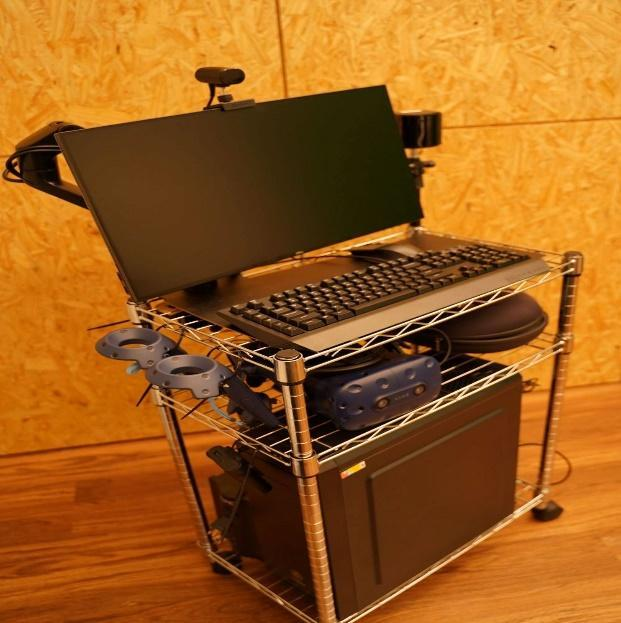
\includegraphics[width=80mm, keepaspectratio]{imgs/image3.jpg}

\columnbreak

\begin{mdframed}[roundcorner=10pt, linecolor=red, linewidth=2pt]
\vspace{1em}
{\Large {\color{red}RISKS}}
\vspace{1em}

\begin{itemize}
    \item Electric Chock;
    \item Equipment Damage;
    \item Physical Damage;
    \item Visual Fatigue; 
\end{itemize}

\vspace{1em}
\end{mdframed}

\vspace{2em}

{\Large Use}
\vspace{1em}

Allowed only with a technician or professor guidance.
\end{multicols}

{\Large Specs}
\vspace{1em}

\textbf{Processor:} Intel i9-9900k 3.6GHz; \textbf{RAM:} 36GB; \textbf{Graphics Card:} NVidia GeForce RTX 2080 TI 11GB VRAM; \textbf{Storage:} 250GB SSD + 2TB HDD;
\newpage

%%%%%%%%%%%%%%%%%%%%%%%%%%%%%%%%%%%%%%%%%%%%%%%%%%%%%%%%%%%%%%%%%%%%%%%%%%%%%%%%%%%%%%%%%%
%%%%%%%%%%%%%%%%%%%%%%%%%%%%%%%%%%%%%%%%%%%%%%%%%%%%%%%%%%%%%%%%%%%%%%%%%%%%%%%%%%%%%%%%%%
%%%%%%%%%%%%%%%%%%%%%%%%%%%%%%%%%%%%%%%%%%%%%%%%%%%%%%%%%%%%%%%%%%%%%%%%%%%%%%%%%%%%%%%%%%
\subsection{Yoke Joystick}
\begin{tabularx}{\textwidth}{ Y  Y  Y  Y }
    \textbf{Description} &  \textbf{Local} &  \textbf{Quantity} & \textbf{Patrimony}\\
    \hline \\
     Demo station & Cart & 1 & Activated
\end{tabularx}
\vspace{1cm}

\begin{multicols}{2}

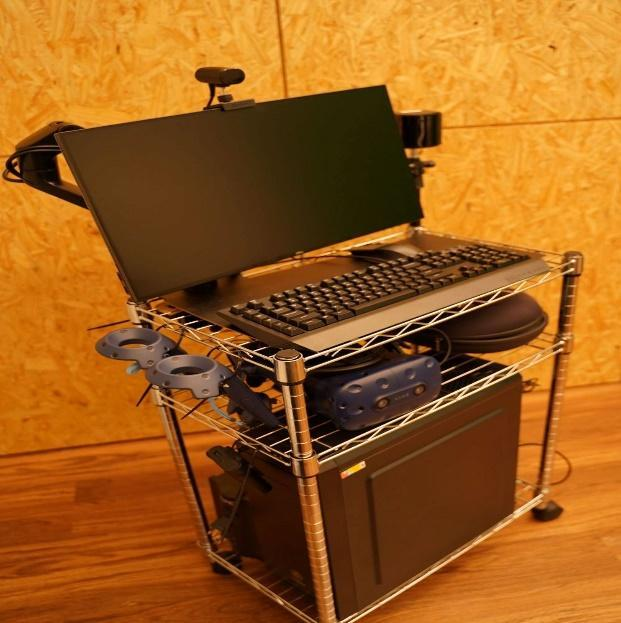
\includegraphics[width=80mm, keepaspectratio]{imgs/image3.jpg}

\columnbreak

\begin{mdframed}[roundcorner=10pt, linecolor=red, linewidth=2pt]
\vspace{1em}
{\Large {\color{red}RISKS}}
\vspace{1em}

\begin{itemize}
    \item Electric Chock;
    \item Equipment Damage;
    \item Physical Damage;
    \item Visual Fatigue; 
\end{itemize}

\vspace{1em}
\end{mdframed}

\vspace{2em}

{\Large Use}
\vspace{1em}

Allowed only with a technician or professor guidance.
\end{multicols}

{\Large Specs}
\vspace{1em}

\textbf{Processor:} Intel i9-9900k 3.6GHz; \textbf{RAM:} 36GB; \textbf{Graphics Card:} NVidia GeForce RTX 2080 TI 11GB VRAM; \textbf{Storage:} 250GB SSD + 2TB HDD;
\newpage


%%%%%%%%%%%%%%%%%%%%%%%%%%%%%%%%%%%%%%%%%%%%%%%%%%%%%%%%%%%%%%%%%%%%%%%%%%%%%%%%%%%%%%%%%%
%%%%%%%%%%%%%%%%%%%%%%%%%%%%%%%%%%%%%%%%%%%%%%%%%%%%%%%%%%%%%%%%%%%%%%%%%%%%%%%%%%%%%%%%%%
%%%%%%%%%%%%%%%%%%%%%%%%%%%%%%%%%%%%%%%%%%%%%%%%%%%%%%%%%%%%%%%%%%%%%%%%%%%%%%%%%%%%%%%%%%
\subsection{Manus VR}
\begin{tabularx}{\textwidth}{ Y  Y  Y  Y }
    \textbf{Description} &  \textbf{Local} &  \textbf{Quantity} & \textbf{Patrimony}\\
    \hline \\
     Demo station & Cart & 1 & Activated
\end{tabularx}
\vspace{1cm}

\begin{multicols}{2}

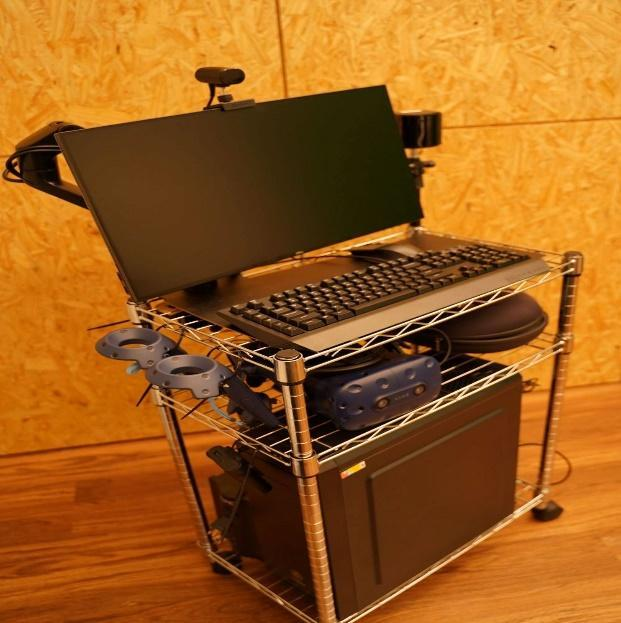
\includegraphics[width=80mm, keepaspectratio]{imgs/image3.jpg}

\columnbreak

\begin{mdframed}[roundcorner=10pt, linecolor=red, linewidth=2pt]
\vspace{1em}
{\Large {\color{red}RISKS}}
\vspace{1em}

\begin{itemize}
    \item Electric Chock;
    \item Equipment Damage;
    \item Physical Damage;
    \item Visual Fatigue; 
\end{itemize}

\vspace{1em}
\end{mdframed}

\vspace{2em}

{\Large Use}
\vspace{1em}

Allowed only with a technician or professor guidance.
\end{multicols}

{\Large Specs}
\vspace{1em}

\textbf{Processor:} Intel i9-9900k 3.6GHz; \textbf{RAM:} 36GB; \textbf{Graphics Card:} NVidia GeForce RTX 2080 TI 11GB VRAM; \textbf{Storage:} 250GB SSD + 2TB HDD;
\newpage


%%%%%%%%%%%%%%%%%%%%%%%%%%%%%%%%%%%%%%%%%%%%%%%%%%%%%%%%%%%%%%%%%%%%%%%%%%%%%%%%%%%%%%%%%%
%%%%%%%%%%%%%%%%%%%%%%%%%%%%%%%%%%%%%%%%%%%%%%%%%%%%%%%%%%%%%%%%%%%%%%%%%%%%%%%%%%%%%%%%%%
%%%%%%%%%%%%%%%%%%%%%%%%%%%%%%%%%%%%%%%%%%%%%%%%%%%%%%%%%%%%%%%%%%%%%%%%%%%%%%%%%%%%%%%%%%
\subsection{EinScan 3D}
\begin{tabularx}{\textwidth}{ Y  Y  Y  Y }
    \textbf{Description} &  \textbf{Local} &  \textbf{Quantity} & \textbf{Patrimony}\\
    \hline \\
     Demo station & Cart & 1 & Activated
\end{tabularx}
\vspace{1cm}

\begin{multicols}{2}

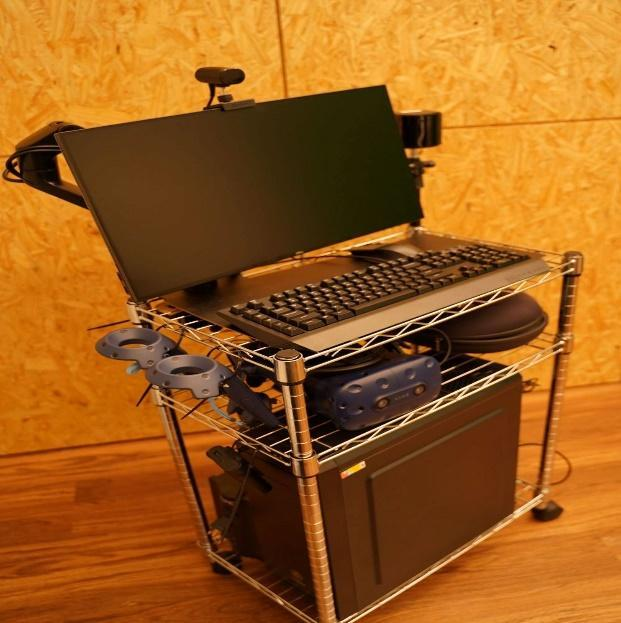
\includegraphics[width=80mm, keepaspectratio]{imgs/image3.jpg}

\columnbreak

\begin{mdframed}[roundcorner=10pt, linecolor=red, linewidth=2pt]
\vspace{1em}
{\Large {\color{red}RISKS}}
\vspace{1em}

\begin{itemize}
    \item Electric Chock;
    \item Equipment Damage;
    \item Physical Damage;
    \item Visual Fatigue; 
\end{itemize}

\vspace{1em}
\end{mdframed}

\vspace{2em}

{\Large Use}
\vspace{1em}

Allowed only with a technician or professor guidance.
\end{multicols}

{\Large Specs}
\vspace{1em}

\textbf{Processor:} Intel i9-9900k 3.6GHz; \textbf{RAM:} 36GB; \textbf{Graphics Card:} NVidia GeForce RTX 2080 TI 11GB VRAM; \textbf{Storage:} 250GB SSD + 2TB HDD;
\newpage


%%%%%%%%%%%%%%%%%%%%%%%%%%%%%%%%%%%%%%%%%%%%%%%%%%%%%%%%%%%%%%%%%%%%%%%%%%%%%%%%%%%%%%%%%%
%%%%%%%%%%%%%%%%%%%%%%%%%%%%%%%%%%%%%%%%%%%%%%%%%%%%%%%%%%%%%%%%%%%%%%%%%%%%%%%%%%%%%%%%%%
%%%%%%%%%%%%%%%%%%%%%%%%%%%%%%%%%%%%%%%%%%%%%%%%%%%%%%%%%%%%%%%%%%%%%%%%%%%%%%%%%%%%%%%%%%
\subsection{VR Cameras}
\begin{tabularx}{\textwidth}{ Y  Y  Y  Y }
    \textbf{Description} &  \textbf{Local} &  \textbf{Quantity} & \textbf{Patrimony}\\
    \hline \\
     Demo station & Cart & 1 & Activated
\end{tabularx}
\vspace{1cm}

\begin{multicols}{2}

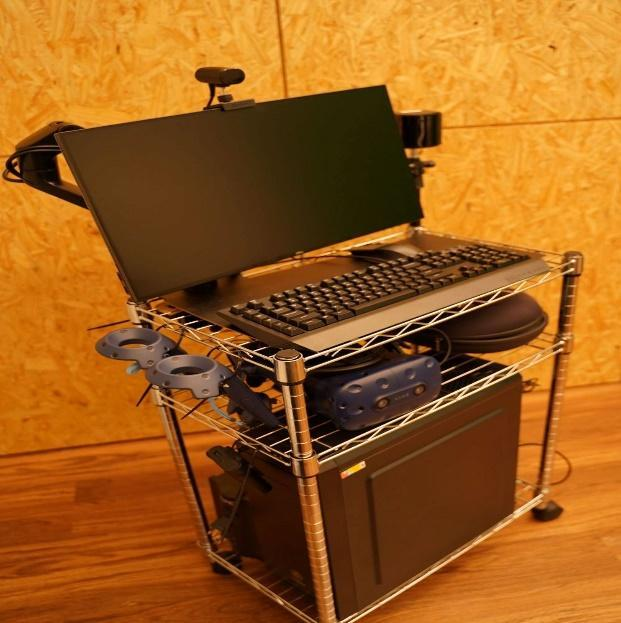
\includegraphics[width=80mm, keepaspectratio]{imgs/image3.jpg}

\columnbreak

\begin{mdframed}[roundcorner=10pt, linecolor=red, linewidth=2pt]
\vspace{1em}
{\Large {\color{red}RISKS}}
\vspace{1em}

\begin{itemize}
    \item Electric Chock;
    \item Equipment Damage;
    \item Physical Damage;
    \item Visual Fatigue; 
\end{itemize}

\vspace{1em}
\end{mdframed}

\vspace{2em}

{\Large Use}
\vspace{1em}

Allowed only with a technician or professor guidance.
\end{multicols}

{\Large Specs}
\vspace{1em}

\textbf{Processor:} Intel i9-9900k 3.6GHz; \textbf{RAM:} 36GB; \textbf{Graphics Card:} NVidia GeForce RTX 2080 TI 11GB VRAM; \textbf{Storage:} 250GB SSD + 2TB HDD;
\newpage

%%%%%%%%%%%%%%%%%%%%%%%%%%%%%%%%%%%%%%%%%%%%%%%%%%%%%%%%%%%%%%%%%%%%%%%%%%%%%%%%%%%%%%%%%%
%%%%%%%%%%%%%%%%%%%%%%%%%%%%%%%%%%%%%%%%%%%%%%%%%%%%%%%%%%%%%%%%%%%%%%%%%%%%%%%%%%%%%%%%%%
%%%%%%%%%%%%%%%%%%%%%%%%%%%%%%%%%%%%%%%%%%%%%%%%%%%%%%%%%%%%%%%%%%%%%%%%%%%%%%%%%%%%%%%%%%
\subsection{Digital Screen Tablet}
\begin{tabularx}{\textwidth}{ Y  Y  Y  Y }
    \textbf{Description} &  \textbf{Local} &  \textbf{Quantity} & \textbf{Patrimony}\\
    \hline \\
     Demo station & Cart & 1 & Activated
\end{tabularx}
\vspace{1cm}

\begin{multicols}{2}

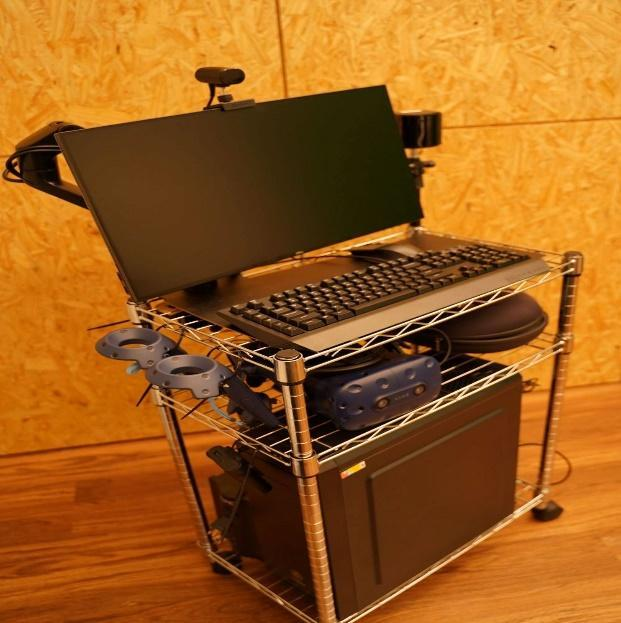
\includegraphics[width=80mm, keepaspectratio]{imgs/image3.jpg}

\columnbreak

\begin{mdframed}[roundcorner=10pt, linecolor=red, linewidth=2pt]
\vspace{1em}
{\Large {\color{red}RISKS}}
\vspace{1em}

\begin{itemize}
    \item Electric Chock;
    \item Equipment Damage;
    \item Physical Damage;
    \item Visual Fatigue; 
\end{itemize}

\vspace{1em}
\end{mdframed}

\vspace{2em}

{\Large Use}
\vspace{1em}

Allowed only with a technician or professor guidance.
\end{multicols}

{\Large Specs}
\vspace{1em}

\textbf{Processor:} Intel i9-9900k 3.6GHz; \textbf{RAM:} 36GB; \textbf{Graphics Card:} NVidia GeForce RTX 2080 TI 11GB VRAM; \textbf{Storage:} 250GB SSD + 2TB HDD;
\newpage


%%%%%%%%%%%%%%%%%%%%%%%%%%%%%%%%%%%%%%%%%%%%%%%%%%%%%%%%%%%%%%%%%%%%%%%%%%%%%%%%%%%%%%%%%%
%%%%%%%%%%%%%%%%%%%%%%%%%%%%%%%%%%%%%%%%%%%%%%%%%%%%%%%%%%%%%%%%%%%%%%%%%%%%%%%%%%%%%%%%%%
%%%%%%%%%%%%%%%%%%%%%%%%%%%%%%%%%%%%%%%%%%%%%%%%%%%%%%%%%%%%%%%%%%%%%%%%%%%%%%%%%%%%%%%%%%
\subsection{Smartphones}
\begin{tabularx}{\textwidth}{ Y  Y  Y  Y }
    \textbf{Description} &  \textbf{Local} &  \textbf{Quantity} & \textbf{Patrimony}\\
    \hline \\
     Demo station & Cart & 1 & Activated
\end{tabularx}
\vspace{1cm}

\begin{multicols}{2}

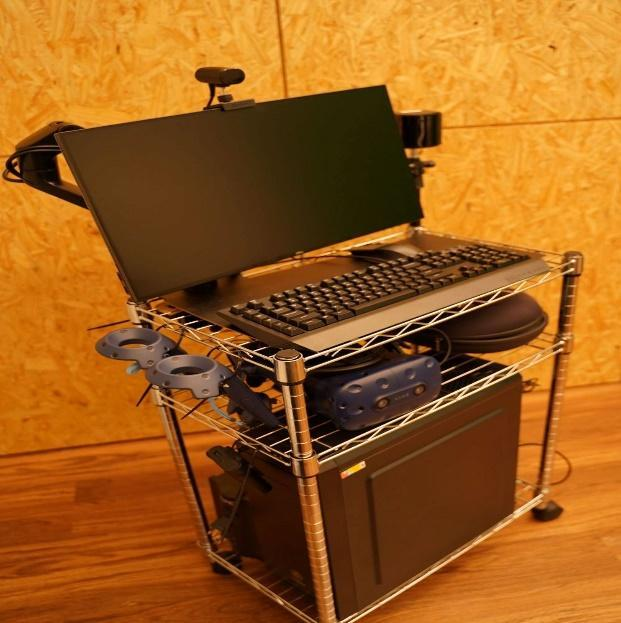
\includegraphics[width=80mm, keepaspectratio]{imgs/image3.jpg}

\columnbreak

\begin{mdframed}[roundcorner=10pt, linecolor=red, linewidth=2pt]
\vspace{1em}
{\Large {\color{red}RISKS}}
\vspace{1em}

\begin{itemize}
    \item Electric Chock;
    \item Equipment Damage;
    \item Physical Damage;
    \item Visual Fatigue; 
\end{itemize}

\vspace{1em}
\end{mdframed}

\vspace{2em}

{\Large Use}
\vspace{1em}

Allowed only with a technician or professor guidance.
\end{multicols}

{\Large Specs}
\vspace{1em}

\textbf{Processor:} Intel i9-9900k 3.6GHz; \textbf{RAM:} 36GB; \textbf{Graphics Card:} NVidia GeForce RTX 2080 TI 11GB VRAM; \textbf{Storage:} 250GB SSD + 2TB HDD;
\newpage
